\section{Results}
% TODO edit here
The EBEs obtained from the EOM and AFQMC calculations are summarized in Table~\ref{tab:EOM}, and the results from the various DMC calculations are summarized in Table~\ref{tab:DMC}.
We consider first the results obtained for R = \SI{4}{\angstrom}, for which HF calculations do not bind the excess electron. 

\subsection{Results for R = \SI{4}{\angstrom}: the correlation bound region}
From Table~\ref{tab:EOM}, it is seen that the EOM-CCSD/aug-cc-pVTZ+7s7p calculations give a value of the EBE of 181 meV for the \ce{(H2O)4} cluster model at R = \SI{4}{\angstrom}.
This increases to 196 meV with the EOM-CCSD(T)(a)$^*$ method.
The AFQMC calculations using the same basis set and for the anion a single determinant of NOs from the restricted SDCI calculation for the trial wave function produce an EBE value of 194 $\pm$ 10 meV, comparable to the EOM-CCSD(T)(a)$^*$ result. 
The EOM-CCSD(T)(a)$^*$ and EOM-CCSDT EBE values calculated with this basis set are nearly identical, demonstrating that the approximate treatment of triples in the former procedure introduces a negligible error in the EBE.
The contribution of supplemental diffuse functions was checked using the EOM-CCSD(T)(a)$^*$ method and the aug-cc-pVTZ+3s1p2d basis set.
These calculations reveal that the inclusion of the supplemental diffuse d functions leads to a $\sim$10 meV increase in the EBE. With the inclusion of this correction, we obtain an estimated EOM-CCSDT EBE of 212 meV. It is expected that the inclusion of the supplemental d functions in the basis set used for the AFQMC calculations would lead to a similar increase in the EBE obtained using that method.

The restricted SDCI procedure, by itself, is not expected to give an accurate value of the EBE and is designed to generate appropriate trial wave functions for DMC or AFQMC calculations on the anion.
In fact, the EBE resulting from the HF treatment of the neutral and the restricted SDCI treatment of the anion using the aug-cc-pVTZ+7s7p basis set is 345 meV, appreciably larger than the EOM and AFQMC values.
This over-binding is due in part to the fact that the restricted SDCI wave function, like the HF wave function, overestimates the magnitude of the dipole moment of the water molecules, resulting in a too favorable electrostatic interaction.
We also constructed a single determinant trial wave function for the anion using the natural orbitals of the restricted SDCI expansion.
We note also that the single determinant of NOs generated from the restricted SDCI wave function and using the aug-cc-pVTZ+7s7p basis set places the anion 160 meV above the neutral when the latter is treated in the HF approximation. 
This is not surprising since this calculation neglects correlation effects other than those incorporated in the determination of the orbitals.
What is important is that the approaches based on the restricted SDCI procedure provide a realistic description of the orbital occupied by the excess electron and avoid the collapse onto the discretized continuum as was observed with the HOMO in the HF calculations. 

% checked by shiv 9/24/20 14:16
\begin{table}[ht!]
    \caption{\label{tab:EOM} EBEs of the \ce{(H2O)4} model calculated using HF, EOM, and AFQMC methods and employing the aug-cc-pVTZ+7s7p basis set.}
\begin{threeparttable}
\begin{tabular}{lr}
Method & EBE (meV)                               \\
\hline
\multicolumn{2}{c}{R = \SI{4.0}{\angstrom}}     \\ 
HF            & -0.4        \\
EOM-CCSD      & 180.6          \\
EOM-CCSD(T)(a)$^*$ & 195.8          \\
    EOM-CCSDT     & 197.5\tnote{1}
    (212.0)\tnote{2} \\
AFQMC SD/HF(N)//SD/NO SDCI(A)     & 194 $\pm$ 10 \\ \hline
\multicolumn{2}{c}{R = \SI{7.0}{\angstrom}}                    \\ 
HF            & 41.3        \\
EOM-CCSD      & 140.2    \\
EOM-CCSD(T)(a)$^*$ & 141.7    \\
EOM-CCSDT    & 143.3\tnote{1}  (154.2)\tnote{2}     \\
AFQMC SD/HF     & 181 $\pm$ 5 \\ 
\end{tabular}
\begin{tablenotes}
\item[1] This EOM-CCSDT/aug-cc-pVTZ+7s7p value was estimated by adding the difference of EBEs from the EOM-CCSD(T)(a)$^*$ and eom-ccsdt calculations with the aug-cc-pVDZ+3s1p basis set to the value from EOM-CCSD(T)(a)$^*$/aug-cc-pVTZ+7s7p.
\item[2] The EOM-CCSDT/aug-cc-pVTZ+7s7p3d value was estimated by adding the difference between the EBEs calculated with the eom-ccsdpt(a)$^*$ with the aug-cc-pVTZ+3s1p and aug-cc-pVTZ+3s1p3d basis sets to the eom-ccsdt/aug-cc-pVTZ+7s7p estimated value in footnote [1] to assess the effect of incorporating diffuse d functions into the basis.
\end{tablenotes}
\end{threeparttable}
\end{table}

In light of the close agreement between the EOM-CCSD(T)(a)$^*$ and AFQMC values of the EBE of the \ce{(H2O)4} model at R = \SI{4}{\angstrom}, when using a comparable basis sets in the two approaches it is relevant to determine whether DMC calculations with sufficiently flexible trial wave functions give an EBE close to the AFQMC and EOM values consistent with these results.
DMC calculations using HF trial wave functions together with the aug-cc-pVDZ/ccECP+7s7p basis set give an EBE of 183 $\pm$ 10 meV, appreciably smaller than the EOM-CCSD(T)(a)$^*$ and AFQMC values.
Interestingly, essentially the same EBE is obtained from the DMC calculations using a Slater determinant of HF orbitals expanded in the aug-cc-pVDZ/ccECP basis set without the 7s7p supplemental set of diffuse functions.
However, if the aug diffuse functions are also removed, the DMC calculations fail to bind the excess electron.
We believe that this is a consequence of the fact that with the cc-pVDZ basis set there is a near zero probability of sampling regions of space at large distances from the molecule, which are important for describing the charge distribution of the excess electron.
% checked by SU and AD 9/24/20 18:31
\begin{table}
    \begin{threeparttable}
        \caption{\label{tab:DMC} EBEs of the \ce{(H2O)4} model calculated using the DMC method and various trial wave functions.\tnote{1}}
    \begin{tabular}{llr}
wave function                  & basis set        &  EBE (meV) \\ \hline
\multicolumn{3}{c}{R = \SI{4.0}{\angstrom}}               \\ 
SD/HF                         & aug-cc-pVDZ+7s7p &  183 $\pm$ 10 \\
SD/HF                         & aug-cc-pVDZ      &  176 $\pm$ 12 \\
SD/HF                         & cc-pVDZ          & -528 $\pm$ 25 \\ 
SD/B3LYP                      & aug-cc-pVDZ+7s7p &  212 $\pm$ 11 \\
SD/HF(N)//SD/NO SDCI(A)    & aug-cc-pVDZ+7s7p &  205 $\pm$ 10 \\
SD/HF(N)//MD/NO SDCI(A)    & aug-cc-pVDZ+7s7p &  202 $\pm$ 12 \\
MD/CIPSI NO                   & aug-cc-pVDZ+3s1p &  190 $\pm$ 9  \\ \hline
\multicolumn{3}{c}{R = \SI{7.0}{\angstrom}}                    \\ 
SD/HF                         & aug-cc-pVDZ+7s7p &   141 $\pm$ 14 \\ 
SD/B3LYP                      & aug-cc-pVDZ+7s7p &   164 $\pm$ 9 \\
SD/HF(N)//SD/NO SDCI(A)    & aug-cc-pVDZ+7s7p &  160 $\pm$ 9 \\
MD/CIPSI NO                   & aug-cc-pVDZ+3s1p &    159 $\pm$ 8 \\
\end{tabular}
\begin{tablenotes}
  \item [1] SD/X indicates that the trial wave function employed a single Slater determinant with X (either HF or B3LYP) orbitals. When different types of trial wave functions are used for the neutral (N) and anion (A) this is indicated by the double slash.
\end{tablenotes}
\end{threeparttable}
\end{table}

A significantly larger value of the EBE is obtained from SD DMC calculations using B3LYP orbitals in place of HF orbitals.
The resulting EBE of 212 $\pm$ 11 meV, within statistical error, agrees with the EOM-CCSD(T)(a)$^{*}$ and AFQMC values.
A similar value of the EBE is obtained from DMC calculations using a single determinant of HF orbitals for the neutral cluster and a single determinant of natural orbitals from the restricted SDCI procedure described in Section~\ref{subsec:rSDCI} for the anion.
DMC calculations using a SD of HF orbitals for trial wave function of the neutral and a trial wave function for the anion retaining 1,392 of the most important determinants from the restricted SDCI calculation gives an EBE of 202 $\pm$ 12 meV, close to the values obtained using the single determinants B3LYP orbitals or of NOs from the SDCI calculation (for the anion). 
The DMC value of the EBE resulting from the anionic trial wave function using a SD of NOs from the restricted SDCI MD calculation results is 205 $\pm$ 10meV, similar to that from DMC calculations using as trial wave functions the MD restricted SDCI wave function for the anion and the HF wave function for the neutral.

Figure~\ref{fig:orbitalsR4} compares the radial charge distributions of the singly occupied orbital from the HF and B3LYP calculations on the excess electron system as well as of the NOs associated with the excess electron from EOM-CCSD, restricted SDCI and CIPSI calculations. 
The collapse of the singly occupied orbital from the HF calculations onto a discretized continuum orbital is readily apparent. 
In contrast, the NOs from the EOM-CCSD and restricted SDCI calculations and the singly occupied orbital from the B3LYP calculation on the anion are more localized and are qualitatively similar to one another. 
These results are consistent with the nodal surface for the anion being significantly improved when using a SD trial wave function that has a physically reasonable charge distribution for the orbital occupied by the excess electron.
Thus, although DMC calculations do recover from the collapse of the HF trial wave function onto a discretized continuum solution in the case of the anion, starting with such a trial function leads to a greater nodal surface error for the anion than for the neutral cluster.
However, we also note that the radial distribution function of the singly occupied orbital from the B3LYP calculation on the anion has a spurious peak near 25 atomic units from the center of the cluster.
This is likely a consequence of the self-interaction error in the B3LYP functional.
The relevant NO extracted from the CIPSI calculations, which were carried using B3LYP orbitals, exhibits a similar shoulder.


\begin{figure}
    \caption{\label{fig:orbitalsR4} Radially integrated charge densities of the singly occupied orbitals from HF and B3LYP calculations and the singly occupied natural orbital from EOM-CCSD, SDCI, and CIPSI calculations  of the model (\ce{(H2O)4}) cluster anion at R = \SI{4}{\angstrom}. All plots generated using Matplotlib.\cite{10.1109/MCSE.2007.55}}.
    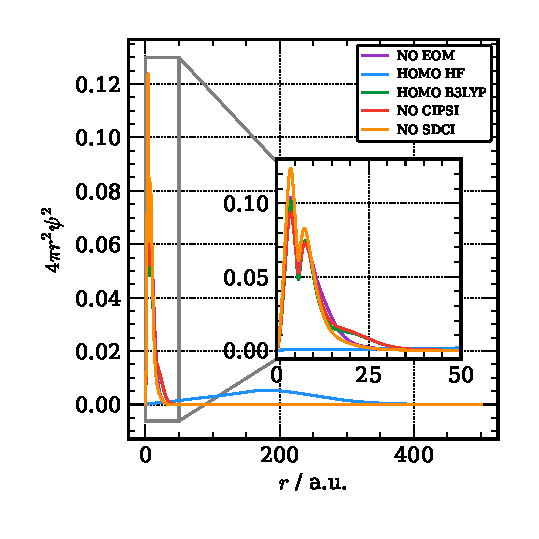
\includegraphics[width=\columnwidth,keepaspectratio]{Images/chapter3/r4_orbitalr2.eps}
\end{figure}


Our final set of DMC calculations at R = \SI{4}{\angstrom} used MD trial wave functions determined from CIPSI calculations for the neutral and anionic clusters. 
The strategy used in performing the CIPSI calculations was presented in Section \ref{subsec:rSDCI}, where it was noted that these calculations, unlike those with the restricted SDCI wave functions, allow for the correlation between the valence electrons change due to the the presence of the excess electron. 
The DMC calculations using the CIPSI trial wave function resulted 190 $\pm$ 9 meV for R = \SI{4}{\angstrom}, slightly under-binding compared to the single determinant DMC value of the EBE obtained using B3LYP orbitals though in close agreement with the results of DMC calculations carried out with the restricted SDCI trial wave function.

\subsection{Results for R = \SI{7}{\angstrom}: the electrostatically bound region}

We now consider the results obtained for the \ce{(H2O)4} cluster model at R = \SI{7}{\angstrom}, for which HF calculations with the aug-cc-pVTZ+7s7p basis set bind the excess electron by 41 meV.
In this case, the EOM-CCSD and EOM-CCSD(T)(a)$^{*}$ calculations give EBEs of 140 meV and 142 meV, respectively.
Thus unlike the situation for R = \SI{4}{\angstrom}, the inclusion of triples in the EOM-CC procedure is relatively unimportant at R = \SI{7}{\angstrom}.
The DMC calculations using SD HF trial wave functions give an EBE of 141 $\pm$ 14 meV, while the DMC calculations using as trial wave functions single determinants of B3LYP orbitals, single determinants generated using the restricted SDCI procedure, or MD trial wavefunctions generated using the CIPSI procedure give similar EBEs values ranging  from 159 $\pm$ 8 to 164 $\pm$ 9 meV. 

Since the anion is bound in the HF approximation at R = \SI{7}{\angstrom}, we also were able to calculate EBEs using separate, frozen-core coupled-cluster calculations for the neutral and anion with the following coupled-cluster methods: coupled-cluster singles, doubles, and a perturbative treatment of triples $\Delta$CCSD(T)\cite{10.1016/S0009-26148987395-6}, coupled-cluster singles, doubles, and triples ($\Delta$CCSDT)\cite{10.1063/1.5128795,10.1063/1.452353,10.1016/0009-26148880110-6,10.1063/1.459002}, and CCSDT with the perturbative treatment of quadruple excitations ($\Delta$CCSDT(Q))\cite{10.1063/1.1950567} methods.
The $\Delta$ indicates that the EBE is derived from the energy difference between the separate calculations on the neutral and anion. The $\Delta$CCSDT and $\Delta$CCSDT(Q) calculations were carried out with only the aug-cc-pVDZ+3s1p basis set.
These calculations indicate that full treatment of the triples, and even approximate treatment of the quadruple excitation contributions, has less than a 1 meV effect on the EBE of the \ce{(H2O)4} cluster model at R = \SI{7.0}{\angstrom}.
On the other hand, the inclusion of diffuse d function in the supplemental set of functions leads to a 12 meV increase in the EBE. With this correction we obtain an estimated EOM-CCSDT EBE of 154 meV, which is in good agreement with the DMC results using suitable trial wave functions.

The AFQMC calculations give an EBE of 181 $\pm$ 5 meV, significantly larger than the EOM-CC results or DMC values.
This most likely reflects an inadequacy of the HF wave function used for the anion in the AFQMC calculations.
Support for this interpretation is provided by examination of Figure~\ref{fig:orbitalsR7}, which shows the radial charge distribution of the excess electron for the \ce{(H2O)4} model at R = \SI{7}{\angstrom}.
From this figure it is seen that although that the HF wave function has not collapsed onto the continuum as it did in the R = \SI{4}{\angstrom} cluster, it is still much more diffuse than that from calculations that include correlation effects. It is also seen from comparisons of Figures~\ref{fig:orbitalsR4} and \ref{fig:orbitalsR7} that the charge distribution associated with the NO occupied by the excess electron in the EOM-CCSD calculations for the cluster with R = \SI{7}{\angstrom}, is more radially extended than that at R = \SI{4}{\angstrom}.
Another noticeable difference between the charge density plots for R = \SI{7}{\angstrom} and \SI{4}{\angstrom} is the reduction of the long-range shoulder in the radial charge distribution of the HOMO from the B3LYP calculations on the anion and in the relevant NO from the CIPSI calculations on the anion carried out using B3LYP orbitals, suggesting that self-interaction errors are less problematical at R = \SI{7}{\angstrom}.

 
\begin{figure}
    \caption{\label{fig:orbitalsR7} Radially integrated charge densities of the singly occupied orbitals from HF and B3LYP calculations and the singly occupied natural orbital from EOM-CCSD, restricted SDCI, and CIPSI calculations  of the model (\ce{(H2O)4}) cluster anion at R = \SI{7}{\angstrom}.}
    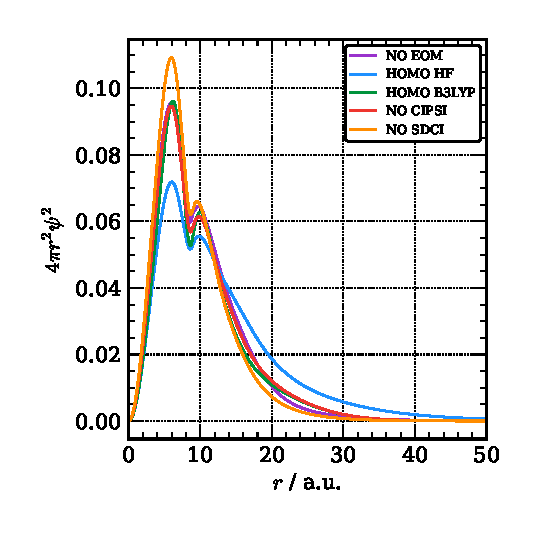
\includegraphics[width=\columnwidth,keepaspectratio]{Images/chapter3/r7_orbitalr2.eps}
\end{figure}

